% Indicate the main file. Must go at the beginning of the file.
% !TEX root = ../main.tex

%----------------------------------------------------------------------------------------
% CHAPTER 3
%----------------------------------------------------------------------------------------

\newtcolorbox{persona}[2][]{
  enhanced,
  raster columns=2,
  colframe=blue!50!black,
  colback=white,
  coltitle=white,
  fonttitle=\bfseries,
  boxed title style={size=small,colframe=red!50!black},
  attach boxed title to top left={yshift=-2mm, xshift=2mm},
  title=#2,#1,
  valign=center,
  boxrule=0.5mm,
  left=5pt,  % Reduced padding on the sides
  right=5pt, % Reduced padding on the sides
  top=5pt,   % Reduced padding on the top
  bottom=5pt, % Reduced padding on the bottom
  boxsep=2pt % Reduced spacing between the border and the content
}


\chapter{Personas}

\label{Chapter3} % For referencing the chapter elsewhere, use \ref{Chapter2} 

\section{Identification of SCRUM Team Roles}

As defined by Mundra \cite{Mundra2013PracticalScrum}, a \ac{SCRUM} team typically comprises four to ten professionals.

\begin{outline}
    \1 \textbf{Product Owner:}
    \2 represents the business
    \3 coordinates requirements
    \3 prioritizes requirements
    \1 \textbf{SCRUM Master:}
    \2 the team coach
    \3 removes impediments faced by team members
    \3 coordination with other teams for any dependencies
    \1 \textbf{Team Members:}
    \2 the developers and testers and others
    \3 involves developers who focus on the technical development
    \3 testers who ensure the product meets quality standards
\end{outline}

\section{Personas for SCRUM Team Roles}

To tailor our proposed approach to the diverse needs within a \ac{SCRUM} team, we introduce detailed personas representing each key role. These personas are designed to guide the development process by highlighting the specific requirements and backgrounds of team members.

\pagebreak

\begin{figure}[h!]
\subsection*{Persona: Emma - Product Owner}
\begin{persona}{Product Owner: Emma}
\begin{tcbraster}[raster columns=2, raster column skip=5mm]
  \begin{tcolorbox}[width=0.2\linewidth, colback=white, colframe=white, boxrule=0pt, halign=center]
    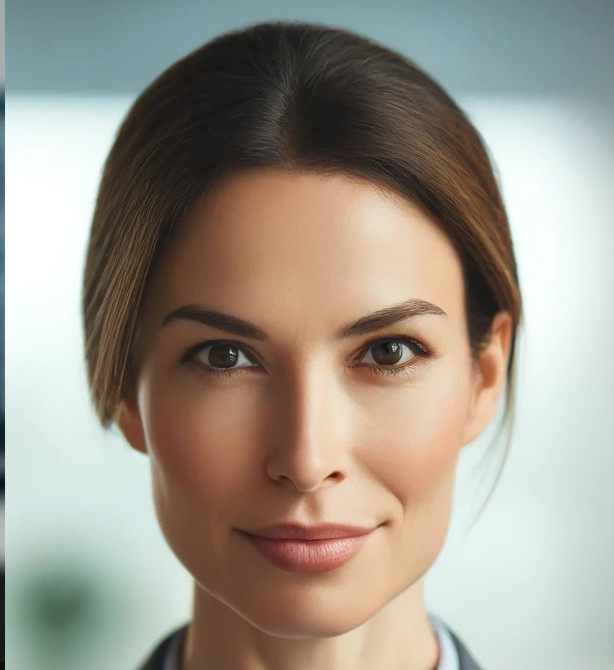
\includegraphics[width=\linewidth, height=6cm, keepaspectratio]{Images/Emma.jpg}
  \end{tcolorbox}
  \begin{tcolorbox}[width=0.8\linewidth, colback=white, colframe=white, boxrule=0pt]
  \fontsize{10pt}{9.6pt}\selectfont
    \textbf{Age:} 38\\
    \textbf{Background:} 
    \begin{itemize}
        \item Background in Product Management
        \item Extensive experience in the technology sector
    \end{itemize}
    \textbf{Needs:}
        \begin{itemize}
        \item High-level overview of project progress
        \item Clear Summaries of technical decisions
    \end{itemize}
  \end{tcolorbox}
\end{tcbraster}
\end{persona}
\caption{Persona with \ac{AI}-Generated Image of Emma, a Product Owner}
\label{fig:persona:emma}
\end{figure}




\begin{figure}[h!]
\subsection*{Persona: Lucas - SCRUM Master}
\begin{persona}{SCRUM Master: Lucas}
\begin{tcbraster}[raster columns=2, raster column skip=5mm]
  \begin{tcolorbox}[width=0.2\linewidth, colback=white, colframe=white, boxrule=0pt, halign=center]
   
\includegraphics[width=\linewidth, height=6cm, keepaspectratio]{Images/Lucas.jpg}
  \end{tcolorbox}
  \begin{tcolorbox}[width=0.8\linewidth, colback=white, colframe=white, boxrule=0pt]
  \fontsize{10pt}{9.6pt}\selectfont
    \textbf{Age:} 33\\
    \textbf{Background:} 
    \begin{itemize}
        \item Certified \ac{SCRUM} Master
        \item Champion of Agile Methodologies
    \end{itemize}
    \textbf{Needs:}
        \begin{itemize}
        \item Tools for workflow management
        \item Tools for performance tracking
        \item Tools for impediment resolution
    \end{itemize}
  \end{tcolorbox}
\end{tcbraster}
\end{persona}
\caption{Persona with \ac{AI}-Generated Image of Lucas, a \ac{SCRUM} Master}
\label{fig:persona:lucas}
\end{figure}

\pagebreak

\begin{figure}[h!]
\subsection*{Persona: Mia - Front-End Developer}
\begin{persona}{Front-End Developer: Mia}
\begin{tcbraster}[raster columns=2, raster column skip=5mm]
  \begin{tcolorbox}[width=0.2\linewidth, colback=white, colframe=white, boxrule=0pt, halign=center]
   
\includegraphics[width=\linewidth, height=6cm, keepaspectratio]{Images/Mia.jpg}
  \end{tcolorbox}
  \begin{tcolorbox}[width=0.8\linewidth, colback=white, colframe=white, boxrule=0pt]
  \fontsize{10pt}{9.6pt}\selectfont
    \textbf{Age:} 29\\
            \textbf{Background:} 
    \begin{itemize}
        \item Specialized in front-end development
        \item works closely with designers to implement engaging user interfaces
        \item work with technologies like HTML, CSS, and Typescript.
    \end{itemize}
    \textbf{Needs:}
        \begin{itemize}
        \item Detailed documentation on \ac{UI}/ \ac{UX} design principles
        \item Documentation for integration with back-end systems
        \item project's visual and functional requirements
    \end{itemize}
  \end{tcolorbox}
\end{tcbraster}
\end{persona}
\caption{Persona with \ac{AI}-Generated Image of Mia, a Front-End Developer}
\label{fig:persona:mia}
\end{figure}

\begin{figure}[h!]
\subsection*{Persona: Alex - Back-End Developer}
\begin{persona}{Back-End Developer: Alex}
\begin{tcbraster}[raster columns=2, raster column skip=5mm]
  \begin{tcolorbox}[width=0.2\linewidth, colback=white, colframe=white, boxrule=0pt, halign=center]
   
\includegraphics[width=\linewidth, height=6cm, keepaspectratio]{Images/Alex.jpg}
  \end{tcolorbox}
  \begin{tcolorbox}[width=0.8\linewidth, colback=white, colframe=white, boxrule=0pt]
  \fontsize{10pt}{9.6pt}\selectfont
    \textbf{Age:} 55\\
    \textbf{Background:} 
    \begin{itemize}
        \item focuses on server-side development
        \item managing databases interfaces
        \item developing application logic in Typescript
        \item proficient in various programming languages and back-end frameworks
    \end{itemize}
    \textbf{Needs:}
        \begin{itemize}
        \item In-depth technical documentation on \ac{API}
        \item system architecture overview
        \item performance optimization guidelines
    \end{itemize}
  \end{tcolorbox}
\end{tcbraster}
\end{persona}
\caption{Persona with \ac{AI}-Generated Image of Alex, a Back-End Developer}
\label{fig:persona:alex}
\end{figure}

\pagebreak

\begin{figure}[h!]
\subsection*{Persona: Klaus - Front-End Developer}
\begin{persona}{Front-End Developer: Klaus}
\begin{tcbraster}[raster columns=2, raster column skip=5mm]
  \begin{tcolorbox}[width=0.2\linewidth, colback=white, colframe=white, boxrule=0pt, halign=center]
   
\includegraphics[width=\linewidth, height=6cm, keepaspectratio]{Images/Klaus.jpg}
  \end{tcolorbox}
  \begin{tcolorbox}[width=0.8\linewidth, colback=white, colframe=white, boxrule=0pt]
  \fontsize{10pt}{9.6pt}\selectfont
    \textbf{Age:} 31\\
            \textbf{Background:} 
    \begin{itemize}
        \item Specialized in front-end development
        \item works closely with designers to implement engaging user interfaces
        \item work with technologies like HTML, CSS, and Typescript.
    \end{itemize}
    \textbf{Needs:}
        \begin{itemize}
        \item Detailed documentation on \ac{UI}/ \ac{UX} design principles
        \item Documentation for integration with back-end systems
        \item project's visual and functional requirements
    \end{itemize}
  \end{tcolorbox}
\end{tcbraster}
\end{persona}
\caption{Persona with \ac{AI}-Generated Image of Klaus, a Front-End Developer}
\label{fig:persona:klaus}
\end{figure}

\begin{figure}[h!]
\subsection*{Persona: Karin - Back-End Developer}
\begin{persona}{Back-End Developer: Karin}
\begin{tcbraster}[raster columns=2, raster column skip=5mm]
  \begin{tcolorbox}[width=0.2\linewidth, colback=white, colframe=white, boxrule=0pt, halign=center]
   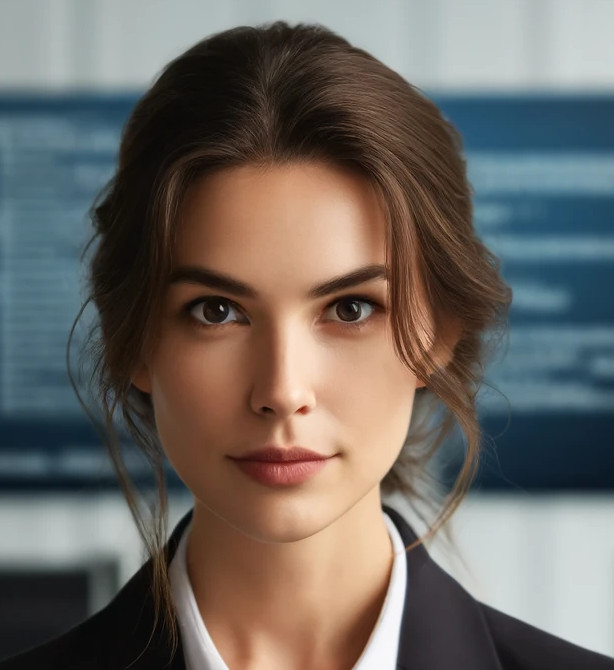
\includegraphics[width=\linewidth, height=6cm, keepaspectratio]{Images/Karin.jpg}
  \end{tcolorbox}
  \begin{tcolorbox}[width=0.8\linewidth, colback=white, colframe=white, boxrule=0pt]
\fontsize{10pt}{9.6pt}\selectfont
    \textbf{Age:} 32\\
    \begin{itemize}
        \item focuses on server-side development
        \item managing databases interfaces
        \item developing application logic in Typescript
        \item proficient in various programming languages and back-end frameworks
    \end{itemize}
    \textbf{Needs:}
        \begin{itemize}
        \item In-depth technical documentation on \ac{API}
        \item system architecture overview
        \item performance optimization guidelines
    \end{itemize}
  \end{tcolorbox}
\end{tcbraster}
\end{persona}
\caption{Persona with \ac{AI}-Generated Image of Karin, a Back-End Developer}
\label{fig:persona:karin}
\end{figure}
\pagebreak




\section{Conclusion}
This chapter has sought to illustrate the composition and dynamics of a \ac{SCRUM} team, through the identification and detailed description of key personas. The distinct roles of the Product Owner, \ac{SCRUM} Master, and various team members are elucidated, in order to demonstrate how these roles collectively contribute to the success of a \ac{SCRUM} project.

The personas presented – Emma (Product Owner), Lucas (\ac{SCRUM} Master), Mia (Front-End Developer), Alex (Back-End Developer), Klaus (Front-End Developer), and Karin (Back-End Developer) – illustrate the diverse backgrounds, needs, and responsibilities within a \ac{SCRUM} team. Each persona highlights the specific expertise and perspectives that are essential for effective teamwork and project management.

The Product Owner, represented by Emma, is responsible for ensuring that the business requirements are prioritised and communicated effectively to the team. Lucas, as the \ac{SCRUM} Master, facilitates \ac{SCRUM} practices and removes impediments, ensuring that the team can function smoothly. The developers, Mia, Alex, Klaus, and Karin, bring their technical skills and collaborate to deliver high-quality software.

The personas demonstrate the value of clear communication, mutual support and the integration of diverse skills and perspectives, which are essential elements of an effective \ac{SCRUM} team. This collaborative approach not only enhances the efficiency and productivity of the team but also fosters a culture of continuous improvement and innovation.

In summary, the detailed personas provide an invaluable practical framework for understanding the roles and interactions within a \ac{SCRUM} team.